\section{Holy Trinity of Variational Principles}\label{sec:variational_principles}
The numerical schemes described in Sec.~\ref{sec:numerical_schemes_for_time_dependent_schrodinger_equation} are theoretically exact, but in practice, they require the representation of the full wavefunction. This is computationally infeasible for large quantum systems due to the exponential growth of grid points required to sample the wavefunction. The variational principles discussed in this section approximate the time evolution by projecting the dynamics onto a lower-dimensional smooth submanifold of the ambient Hilbert space $\mathcal{M}\subset\mathcal{H}$. We define this manifold as the set of all trial wavefunctions parametrized by a complex vector $\symbf{\alpha}(t)\in\mathbb{C}^N$ as
\begin{equation}\label{eq:variational_manifold}
\mathcal{M}=\lbrace\ket{\Psi(\symbf{\alpha})}:\symbf{\alpha}\in\mathbb{C}^N\rbrace,
\end{equation}
where $N$ is the number of parameters and $\ket{\Psi(\symbf{\alpha})}$ is the parametrized wavefunction. This approach allows us to evolve the system's state using a manageable number of parameters $\symbf{\alpha}=(\alpha_1(t),\ldots,\alpha_N(t))$. We assume, that the manifold in Eq.~\eqref{eq:variational_manifold} is holomorphic, i.e. the trial wavefunctions $\ket{\Psi(\symbf{\alpha})}$ do not depend on $\symbf{\alpha}^\ast$ as is the common practice. In the following subsections, we will explore three key variational principles: the Dirac--Frenkel principle, McLachlan's variational principle, and the time-dependent variational principle. Throughout the following sections, we will sometimes use $\Psi:=\ket{\Psi(\symbf{\alpha})}$ to denote the parametrized state vector and $\dot\Psi:=\ddt\ket{\Psi(\symbf{\alpha})}$ to denote its time derivative when appropriate.
\subsection{Dirac--Frenkel Principle}\label{sec:dirac_frenkel_principle}
The first variational principle we consider is the \acrfull{dfvp}.\supercite{10.1017/S0305004100016108,1477741} According to the \acrshort{tdse}, the exact time-derivative vector of the state $\ket{\Psi(\symbf{\alpha})}$ is given by $-\i H\ket{\Psi(\symbf{\alpha})}$. This vector represents the true velocity of the state in the ambient Hilbert space $\mathcal{H}$, dictating how the state evolves over time. However, the vector $-\i H\ket{\Psi(\symbf{\alpha})}$ generally leads out of the manifold $\mathcal{M}$. We therefore seek a time-derivative vector that lies strictly within the tangent space $T_{\Psi}\mathcal{M}$.

Formalizing this, the tangent space of the holomorphic manifold $\mathcal{M}$ at a point $\ket{\Psi(\symbf{\alpha})}$ is spanned by the partial derivatives of the wavefunction with respect to the parameters
\begin{equation}
T_{\Psi}\mathcal{M}=\text{span}\left\lbrace\frac{\partial}{\partial\alpha_k}\ket{\Psi(\symbf{\alpha})}\right\rbrace_{k=1}^N.
\end{equation}
The tangent space $T_{\Psi}\mathcal{M}$ represents all possible directions in which the state $\ket{\Psi(\symbf{\alpha})}$ can evolve while remaining within the manifold $\mathcal{M}$. Consequently, the approximate time evolution of the state is given by the chain rule as
\begin{equation}\label{eq:tangent_evolution}
\ddt\ket{\Psi\left(\symbf{\alpha}\right)}=\sum_{k=1}^N\dot{\alpha}_k\frac{\partial}{\partial\alpha_k}\ket{\Psi(\symbf{\alpha})}\in T_{\Psi}\mathcal{M}.
\end{equation}
The approximate time evolution in Eq.~\eqref{eq:tangent_evolution} represents a velocity vector $\ddt\ket{\Psi\left(\symbf{\alpha}\right)}$ as the state moves through the manifold $\mathcal{M}$, with the parameters $\symbf{\alpha}$ changing at rates $\dot{\symbf{\alpha}}=(\dot{\alpha}_1(t),\ldots,\dot{\alpha}_N(t))$. The goal is to determine the optimal derivatives $\dot{\symbf{\alpha}}$ that best approximate the true dynamics dictated by the \acrshort{tdse}. The Dirac--Frenkel principle postulates that the optimal parameters $\dot{\symbf{\alpha}}$ are found by minimizing the distance between the exact dynamics and the tangent space evolution. We define the residual vector (the error) as
\begin{equation}\label{eq:dfvp_residual_vector}
\ket{\epsilon}=\ddt\ket{\Psi\left(\symbf{\alpha}\right)}+\i H\ket{\Psi\left(\symbf{\alpha}\right)}=\ket{\dot\Psi+\i H\Psi},
\end{equation}
which quantifies the deviation of the approximate time evolution from the exact dynamics. In an ideal scenario, we would have $\ket{\epsilon}=\ket{0}$, indicating perfect agreement between the approximate and exact evolutions. However, since the tangent space is a restricted to a manifold $\mathcal{M}$, we generally cannot achieve this ideal case. To find the optimal evolution within the restricted manifold, we project the exact time-derivative vector onto the tangent space, as illustrated in Fig.~\ref{fig:dirac_frenkel_principle}.
\begin{figure}[!ht]
\centering
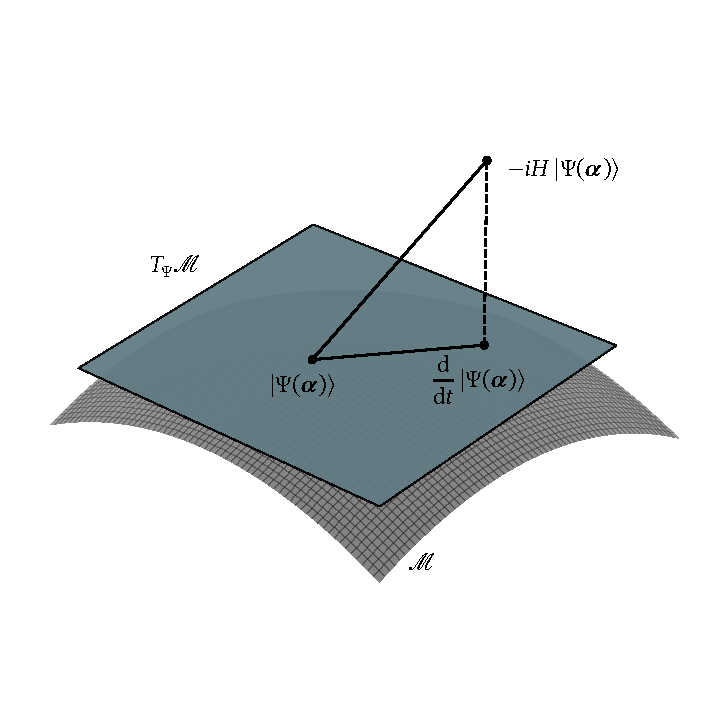
\includegraphics[clip,trim={0.7cm 2.1cm 0.5cm 2.0cm},width=0.6\linewidth]{parts/01-Theoretical_Foundations/chapters/02-Time_Evolution_in_Quantum_Mechanics/sections/images/dfvp_schema}
\caption{The Dirac--Frenkel variational principle projects the exact time-derivative vector $-\i H\ket{\Psi\left(\symbf{\alpha}\right)}$ onto the tangent space $T_{\Psi}\mathcal{M}$ to find the optimal approximate time evolution $\ddt\ket{\Psi\left(\symbf{\alpha}\right)}$. The residual vector $\ket{\epsilon}$ (dashed line) is orthogonal to the tangent space $T_{\Psi}\mathcal{M}$.}
\label{fig:dirac_frenkel_principle}
\end{figure}
Mathematically, this is expressed by the condition that the inner product of the residual vector with any vector in the tangent space $T_{\Psi}\mathcal{M}$ is zero:
\begin{equation}\label{eq:dfvp_orthogonality_condition}
\Braket{\delta\Psi|\dot\Psi+\i H\Psi}=0,
\end{equation}
where $\ket{\delta\Psi}$ represents arbitrary variations within the tangent space. The Eq.~\eqref{eq:dfvp_orthogonality_condition} must hold for all $\ket{\delta\Psi}\in T_{\Psi}\mathcal{M}$ and constitutes the formal definition of the \acrshort{dfvp}, yielding equations of motion for parameters $\symbf{\alpha}$.
\subsection{McLachlan's Variational Principle}\label{sec:mclachlan_variational_principle}
The McLachlan's variational principle offers an alternative approach to approximating the time evolution of a quantum system within a restricted manifold. Instead of projecting the exact time-derivative vector onto the tangent space, McLachlan's principle seeks to minimize the norm of the residual vector $\ket{\epsilon}$ (Eq.~\eqref{eq:dfvp_residual_vector}) directly.\supercite{10.1080/00268976400100041} Mathematically, we write that the variation of the squared norm of the residual vector with respect to the state velocity $\ddt\ket{\Psi\left(\symbf{\alpha}\right)}$ is zero:
\begin{equation}\label{eq:mclachlan_variational_principle_condition}
\delta_{\dot\Psi}\Braket{\epsilon|\epsilon}=\delta_{\dot\Psi}\Braket{\dot\Psi+\i H\Psi|\dot\Psi+\i H\Psi}=0.
\end{equation}
Performing the variation in Eq.~\eqref{eq:mclachlan_variational_principle_condition} leads to the condition
\begin{equation}\label{eq:mclachlan_variational_principle_intermediate}
\Braket{\delta\dot\Psi|\dot\Psi+\i H\Psi}+\Braket{\dot\Psi+\i H\Psi|\delta\dot\Psi}=0.
\end{equation}
One can also recognize that $\ket{\delta\dot\Psi}$ lies within the tangent space $T_{\Psi}\mathcal{M}$, similar to $\ket{\delta\Psi}$ in the Dirac--Frenkel principle since
\begin{equation}\label{eq:tangent_variation_equality}
\ket{\delta\dot\Psi}=\sum_{k=1}^N\delta\dot{\alpha}_k\frac{\partial}{\partial\alpha_k}\ket{\Psi(\symbf{\alpha})}\in T_{\Psi}\mathcal{M}.
\end{equation}
The Eq.~\eqref{eq:mclachlan_variational_principle_intermediate} can be further simplified using Eq.~\eqref{eq:tangent_variation_equality} and recognizing that the second term is the complex conjugate of the first term. Thus, using the property of complex conjugation that $z+z^\ast=2\Re z$ for any complex number $z$, we can rewrite the Eq.~\eqref{eq:mclachlan_variational_principle_intermediate} as\footnote{Note that some authors define McLachlan's error vector as $\ket{\epsilon}=\ket{\i\dot\Psi-H\Psi}$, which is equivalent to our definition up to a global phase factor. This alternative definition leads to a slightly different form of McLachlan's variational principle where the real part operator $\Re$ is replaced by the imaginary part operator $\Im$. However, both forms are mathematically equivalent since $\Re(z)=\Im(\i z)$ for any complex number $z$.}
\begin{equation}\label{eq:mclachlan_variational_principle}
\Re\Braket{\delta\Psi|\dot\Psi+\i H\Psi}=0,
\end{equation}
where we have used the fact that $\ket{\delta\dot\Psi}$ and $\ket{\delta\Psi}$ live in the same tangent space $T_{\Psi}\mathcal{M}$. The Eq.~\eqref{eq:mclachlan_variational_principle} defines McLachlan's variational principle, which aims to find the optimal time evolution within the manifold $\mathcal{M}$ by minimizing the norm of the residual vector $\ket{\epsilon}$. The noticable difference between McLachlan's principle and the Dirac--Frenkel principle (Eq.~\eqref{eq:dfvp_orthogonality_condition}) is the presence of the real part operator $\Re$ in Eq.~\eqref{eq:mclachlan_variational_principle}. This distinction implies that McLachlan's principle focuses on minimizing the overall error magnitude, while the Dirac--Frenkel principle enforces strict orthogonality of the residual vector to the tangent space.

Now the question arises: are these two variational principles (Eq.~\eqref{eq:dfvp_orthogonality_condition} and Eq.~\eqref{eq:mclachlan_variational_principle}) equivalent? Recall that we assumed the manifold $\mathcal{M}$ to be holomorphic, meaning that the trial wavefunctions $\ket{\Psi(\symbf{\alpha})}$ do not depend on the complex conjugates of the parameters $\symbf{\alpha}^\ast$. This assumption ensures that any vector from the tangent space $T_{\Psi}\mathcal{M}$ multiplied by the imaginary unit $\i$ also lies within the tangent space $T_{\Psi}\mathcal{M}$ as follows from Eq.~\eqref{eq:tangent_evolution}. By this logic and the fact that $\Im(z)=\Re(-\i z)$ for any complex number $z$, we get
\begin{equation}\label{eq:mclachlan_dfvp_equivalence}
\Re\left(-\i\Braket{\delta\Psi|\dot\Psi+\i H\Psi}\right)=\Im\Braket{\delta\Psi|\dot\Psi+\i H\Psi}=0,
\end{equation}
which shows that the Dirac--Frenkel principle (Eq.~\eqref{eq:dfvp_orthogonality_condition}) and McLachlan's principle (Eq.~\eqref{eq:mclachlan_variational_principle}) are indeed equivalent when the manifold $\mathcal{M}$ is holomorphic. Should the manifold $\mathcal{M}$ not be holomorphic, a derivative with respect to $\symbf{\alpha}^\ast$ would appear in the elements of the tangent space $T_{\Psi}\mathcal{M}$, and the Eq.~\eqref{eq:mclachlan_dfvp_equivalence} would no longer hold. In such cases, the two variational principles would yield different equations of motion for the parameters $\symbf{\alpha}$.\supercite{297500112}
\subsection{Time-Dependent Variational Principle}\label{sec:time_dependent_variational_principle}
The third perspective on variational principles is provided by the time-dependent variational principle, which is rooted in the action formalism of classical mechanics. In this approach, we define the Lagrangian as\supercite{10.1088/1742-6596/99/1/012009,7550989}
\begin{equation}\label{eq:dirac_lagrangian}
\mathcal{L}(\symbf{\alpha},\symbf{\alpha}^\ast)=\Braket{\Psi|\i\dot\Psi-H\Psi}.
\end{equation},
where the we have dropped the explicit dependence of the wavefunction on the parameters $\symbf{\alpha}$ for brevity. Should we use a non-parametrized wavefunction $\ket{\Psi(t)}$ and apply the principle of stationary action, we would recover the \acrshort{tdse} (and its conjugate). However, since we are working with a parametrized wavefunction $\ket{\Psi(\symbf{\alpha})}$, we restrict the variations to those allowed by the manifold $\mathcal{M}$. The time-dependent variational principle states that the optimal parameters $\symbf{\alpha}$ are those that make the action functional stationary with action given by the time integral of the Lagrangian
\begin{equation}\label{eq:action_functional}
S(\symbf{\alpha},\symbf{\alpha}^\ast)=\int_{t_0}^{t_1}\mathcal{L}(\symbf{\alpha},\symbf{\alpha}^\ast)\dt.
\end{equation}
Applying the principle of stationary action $\delta S=0$ to the action functional in Eq.~\eqref{eq:action_functional} leads to the Euler--Lagrange equations for the parameter conjugates $\symbf{\alpha}^\ast$
\begin{equation}\label{eq:euler_lagrange_equations}
\ddt\frac{\partial\mathcal{L}}{\partial\dot{\alpha}_k^\ast}-\frac{\partial\mathcal{L}}{\partial\alpha_k^\ast}=0,\quad k=1,\ldots,N.
\end{equation}
Note that taking the variation with respect to the parameter conjugates $\symbf{\alpha}^\ast$ yields equations of motion for the parameters $\symbf{\alpha}$. One can also derive equations of motion for the parameter conjugates $\symbf{\alpha}^\ast$ by applying the principle of stationary action to the parameters $\symbf{\alpha}$ instead. Eq.~\eqref{eq:euler_lagrange_equations} provides a set of coupled differential equations that govern the time evolution of the parameters $\symbf{\alpha}$ within the manifold $\mathcal{M}$. Solving these equations yields the optimal trajectory of the parameters that best approximates the true dynamics of the quantum system while remaining within the constraints of the chosen manifold.

To demonstrate the equivalence of this approach to the Dirac--Frenkel principle for holomorphic manifolds, we explicitly evaluate the terms in Eq.~\eqref{eq:euler_lagrange_equations}. Assuming the parametrization is holomorphic, the ket vector $\ket{\Psi(\symbf{\alpha})}$ depends only on $\symbf{\alpha}$, while the bra vector $\bra{\Psi(\symbf{\alpha})}$ depends only on $\symbf{\alpha}^\ast$. Consequently, the Lagrangian in Eq.~\eqref{eq:dirac_lagrangian} does not explicitly depend on the time derivatives of the conjugate parameters $\dot{\symbf{\alpha}}^\ast$, leading to
\begin{equation}
\frac{\partial\mathcal{L}}{\partial\dot{\alpha}_k^\ast}=0.
\end{equation}
The Euler--Lagrange equations therefore simplify to the condition $\frac{\partial\mathcal{L}}{\partial\alpha_k^\ast}=0$. Plugging in the Lagrangian from Eq.~\eqref{eq:dirac_lagrangian} leads to
\begin{equation}\label{eq:tdvp_derivation}
\frac{\partial\mathcal{L}}{\partial\alpha_k^\ast}=\frac{\partial}{\partial\alpha_k^\ast}\Braket{\Psi|\i\dot\Psi-H\Psi}=0.
\end{equation}
Since $\frac{\partial}{\partial\alpha_k}\ket{\Psi}$ spans the tangent space $T_{\Psi}\mathcal{M}$ the condition holding for all $k$ implies it holds for any arbitrary variation $\ket{\delta\Psi}$ and we can rewrite Eq.~\eqref{eq:tdvp_derivation} as
\begin{equation}
\Braket{\delta\Psi|\i\dot\Psi-H\Psi}=0\implies\Braket{\delta\Psi|\dot\Psi+\i H\Psi}=0,
\end{equation}
hence recovering the Dirac--Frenkel variational principle (Eq.~\eqref{eq:dfvp_orthogonality_condition}). This demonstrates that the time-dependent variational principle is equivalent to the Dirac--Frenkel principle when the manifold $\mathcal{M}$ is holomorphic.
